% Preamble
% ---
\documentclass{article}

% Packages
% ---
\usepackage{amsmath} % Advanced math typesetting
\usepackage[utf8]{inputenc} % Unicode support (Umlauts etc.)
\usepackage{hyperref} % Add a link to your document
\usepackage{graphicx} % Add pictures to your document
\usepackage{listings} % Source code formatting and highlighting
\usepackage{float}
\usepackage[margin=2cm]{geometry}


\title{Guia de uso de Lattice Radiant Software}
\date{2019-09-01}
\author{Electronica 3}

\begin{document}

\maketitle
\pagenumbering{gobble}
\newpage
\pagenumbering{arabic}

\section{Introduccion}

\section{Descarga e instalacion}
El software utilizado para programar la FPGA provista por la catedra es 'Lattice Radiant Software'.El mismo puede descargarse tanto para Linux como para Windows del siguiente link: \url{https://tinyurl.com/y46mth4j}

\section{Creacion de un proyecto}
	Para crear un nuevo proyecto se debe abrir el programa recientemente instalado y elegir 'New Project'.
	\begin{figure}[H]
	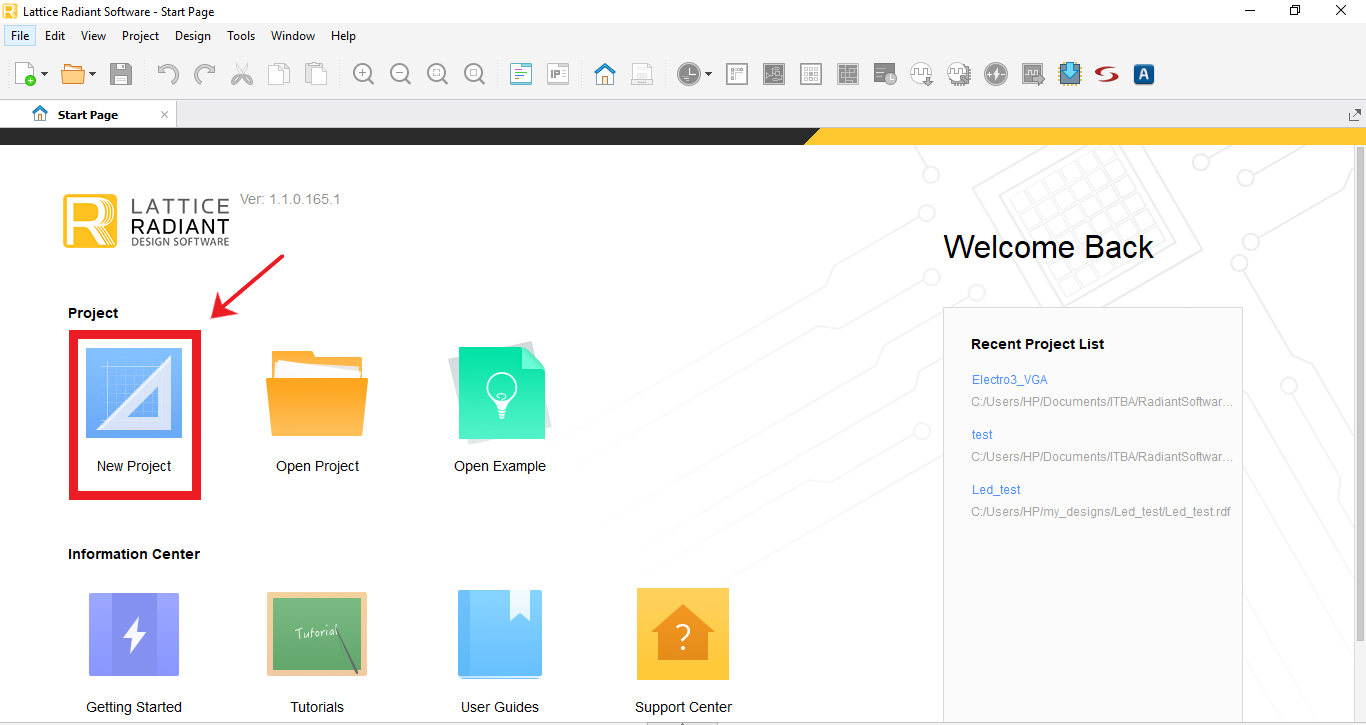
\includegraphics[width=\textwidth]{Imagenes/NewProj.png}
	\caption{Opcion para crear un nuevo proyecto}
	\end{figure}
	
	Luego de hacer click en New Project y en el boton de next, se debe elegir el nombre del proyecto y en que carpeta se desea guardar.Dejar el nombre bajo el campo de "Implementation" en su valor default y hacer click en next nuevamente.
	En la siguiente ventana se puede elegir agregar archivos al nuevo proyecto.En este paso se puede elegir agregar cualquier achivo de Verilog ya existente que sea necesario para el proyecto.
	\begin{figure}[H]
	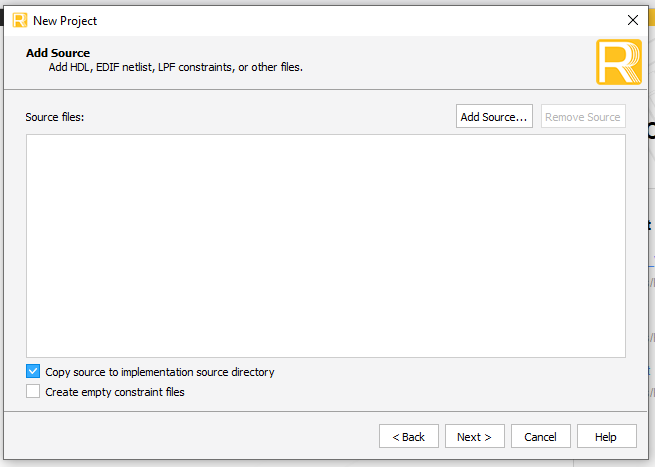
\includegraphics[width=\textwidth]{Imagenes/AddSources.png}
	\caption{Ventana para agregar archivos ya existentes}
	\end{figure}
	
	Tildar las opciones como se indica en la figura anterior y hacer click en Next.
	En la siguiente ventana se indica el dispositivo a utilizar, completar las opciones igual que como se muestra en la siguiente figura:
	\begin{figure}[H]
	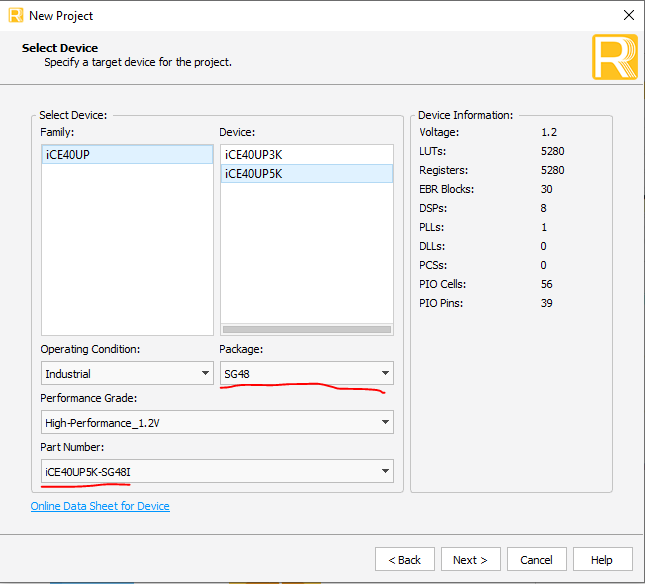
\includegraphics[width=\textwidth]{Imagenes/Dispositivo.png}
	\caption{Prestar especial antencion a que el campo de 'Package' y 'Part Number' coincidan con el de la imagen }
	\end{figure}
	Clickear Next nuevamente, elegir la opcion 'Lattice LSE' en la siguiente ventana, elegir next una vez mas y luego Finish.
	

\subsection{Modulos de Verilog}
\subsection{Constraints}

\section{Simulacion}

\section{Asignacion de pins}
Para asignar que pin de la FPGA corresponde a que entrada y salida del modulo de Verilog, se debe ir al 'Device Constraint Editor'.
	\begin{figure}[H]
	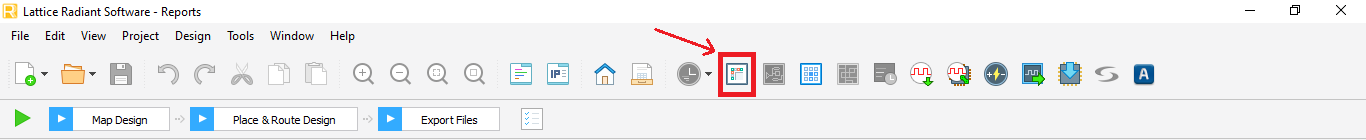
\includegraphics[width=\textwidth]{Imagenes/pins.png}
	\caption{Ubicacion del Device Constraint Editor en el Radiant}
	\end{figure}
	
 Una vez abierto el Device Constraint Editor se vera algo similar a lo observado en la siguiente figura:
 	\begin{figure}[H]
	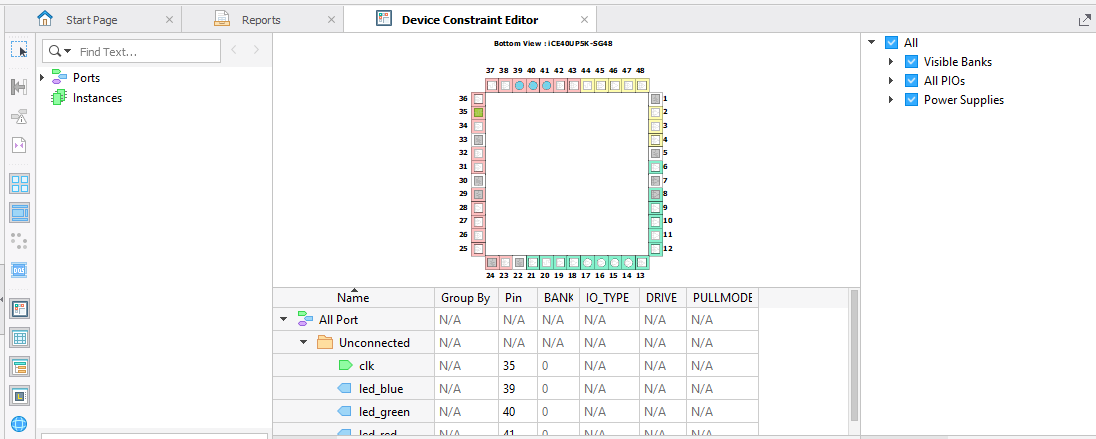
\includegraphics[width=\textwidth]{Imagenes/DeviceConstraintEditor.png}
	\caption{Vista de las senales de Verilog y sus pins correspondientes}
	\end{figure}
 En esta ventana se puede cambiar que pin corresponde a una senal del modulo de Verilog mas alto en la jerarquia.Para realizar cambios solo hace falta hacer click en el campo de 'pin' correspondiente a una senal dada y cambiar el valor numerico.Antes del nombre de cada senal hay una flecha con una direccion y color determinado que indica si la senal es de input o de output.
 
 Hay que tener especial cuidado de asignar pins validos para las senales (utilizar los pins I/O).A continuacion se presentan algunas tablas con la funcion de algunos pins de la FPGA que utiliza la catedra(ICE40-UP5K).
 \begin{figure}[H]
 	\centering
	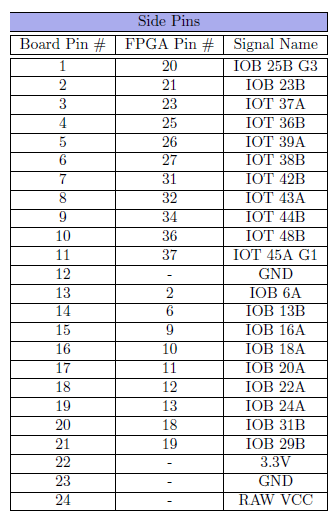
\includegraphics[height=8cm,width=5cm]{Imagenes/SidePins.png}
	\end{figure}
 \begin{figure}[H]
 	\centering
	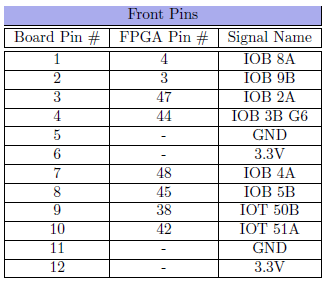
\includegraphics[height=6cm, width=5cm]{Imagenes/FrontPins.png}
	\end{figure}
\section{Esquema de la FPGA}

\section{Compilacion,sintesis y programador}

\end{document}